
%%%%%%%%%%%%%%%%%
%%%%%%%%%%%%%%%%%
\begin{frame}
	\shiftedframetitle{4. Implementation}
\begin{itemize}
 \item \myCRed{Coupling} \& \myCRed{Mapping} data from/to all setups:
 \end{itemize}
  \vspace{0.4cm}
\begin{table}[]
\begin{tabular}{|lll|}\hline
$2D$ SWE       & $\rightarrow$ & $2D$ SWE       \\ \hline
$2D$ SWE       & $\rightarrow$ & $3D$ OpenFOAM \\ \hline
$3D$ OpenFOAM & $\rightarrow$ & $2D$ SWE       \\ \hline
$3D$ OpenFOAM & $\rightarrow$ & $3D$ OpenFOAM \\ \hline
\end{tabular}
\caption{Mapping setups}
\label{table:1}
\end{table}
\end{frame}


\begin{frame}
%TODO improve this slide
\shiftedframetitle{\large Boundary Conditions}
\begin{figure}
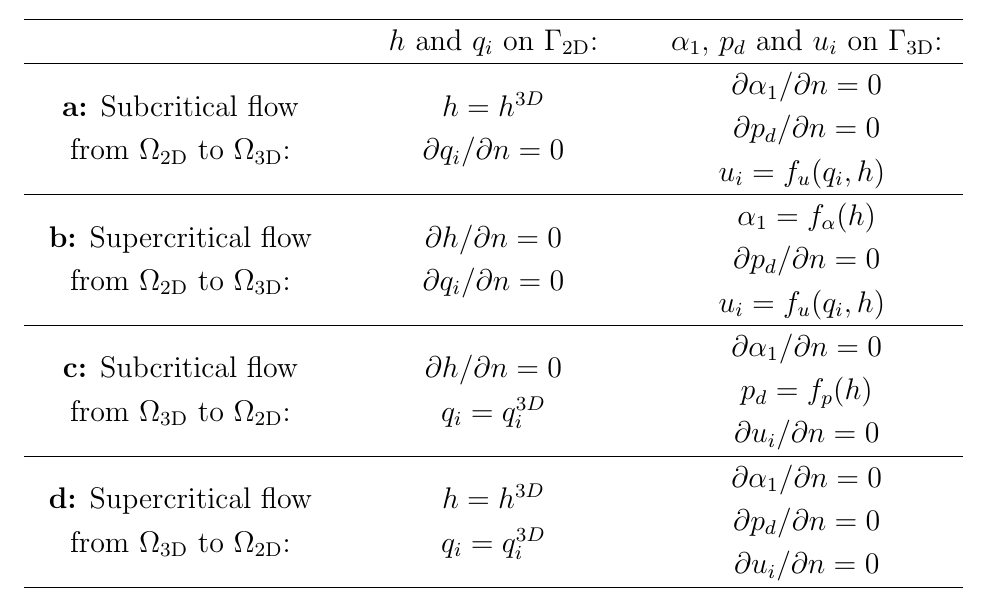
\includegraphics[scale=0.44]{./Resources/Images/bcs_mintgen.png}
\caption{Boundary condition used by \cite{mintgen}}
\end{figure}
\end{frame}

